\documentclass{beamer}

\usepackage{amssymb,amsmath}
\usepackage{graphicx}
\usepackage{url}
\usepackage{color}
\usepackage{pagenote}[continuous,page]
\usepackage{relsize}		% For \smaller
\usepackage{url}			% For \url
\usepackage{epstopdf}	% Included EPS files automatically converted to PDF to include with pdflatex

%For MindMaps
% \usepackage{tikz}%
% \usetikzlibrary{mindmap,trees,arrows}%

%%% Color Definitions %%%%%%%%%%%%%%%%%%%%%%%%%%%%%%%%%%%%%%%%%%%%%%%%%%%%%%%%%
%\definecolor{bordercol}{RGB}{40,40,40}
%\definecolor{headercol1}{RGB}{186,215,230}
%\definecolor{headercol2}{RGB}{80,80,80}
%\definecolor{headerfontcol}{RGB}{0,0,0}
%\definecolor{boxcolor}{RGB}{186,215,230}

%%% Save space in lists. Use this after the opening of the list %%%%%%%%%%%%%%%%
%\newcommand{\compresslist}{
%	\setlength{\itemsep}{1pt}
%	\setlength{\parskip}{0pt}
%	\setlength{\parsep}{0pt}
%}

%\setbeameroption{show notes on top}

% You should run 'pdflatex' TWICE, because of TOC issues.

% Rename this file.  A common temptation for first-time slide makers
% is to name it something like ``my_talk.tex'' or
% ``john_doe_talk.tex'' or even ``discrete_math_seminar_talk.tex''.
% You really won't like any of these titles the second time you give a
% talk.  Try naming your tex file something more descriptive, like
% ``riemann_hypothesis_short_proof_talk.tex''.  Even better (in case
% you recycle 99% of a talk, but still want to change a little, and
% retain copies of each), how about
% ``riemann_hypothesis_short_proof_MIT-Colloquium.2000-01-01.tex''?

\mode<presentation>
{
  \usetheme{CambridgeUS}		% bem bacana - menu superior
  \usecolortheme{default}		% branco, azul clarinho
  \useoutertheme{default}
  \useinnertheme{circles}
  \setbeamercovered{invisible}
}

\beamertemplatenavigationsymbolsempty

%% Better looking blocks
\setbeamercolor{block title alerted}{use=structure,fg=black,bg=red!80!black}
\setbeamercolor{block body alerted}{use=structure,fg=black,bg=white!90!black}

\setbeamercolor{block title}{use=structure,fg=black,bg=blue!60!white}
\setbeamercolor{block body}{use=structure,fg=black,bg=white!90!black}

\usepackage[english]{babel}
\usepackage[latin1]{inputenc}
\usepackage{subfigure}

\usepackage{times}
\usepackage[T1]{fontenc}

%% makes the ppagenote command for figure references at the end.
\makepagenote
\renewcommand{\notenumintext}[1]{}
\newcommand{\ppagenote}[1]{\pagenote[Page \insertframenumber]{#1}}


\usepackage{tikz}
\usetikzlibrary{arrows,shapes}

\title[GB13604]{GB13604 - Maths for Computer Science}
\subtitle[]{Lecture 10 -- Probability, Part III}
\author[CC-BY-NC-SA]{Claus Aranha\\{\footnotesize caranha@cs.tsukuba.ac.jp}}
\institute[]{College of Information Science}
\date[2018-12-19]{2018-12-19\\{\tiny Last updated \today}}

\tikzstyle{vertex}=[circle,fill=black!25,minimum size=10pt,inner sep=0pt]
\tikzstyle{blue vertex}=[circle,fill=blue!100,minimum size=10pt,inner sep=0pt]
\tikzstyle{red vertex}=[circle,fill=red!100,minimum size=10pt,inner sep=0pt]
\tikzstyle{yellow vertex}=[circle,fill=yellow!100,minimum size=10pt,inner sep=0pt]
\tikzstyle{edge} = [draw,thick,-]
\tikzstyle{pedge} = [draw,thick,.]
\tikzstyle{red edge} = [draw, thick,-,red!50]
\tikzstyle{black edge} = [draw, line width=2pt,-,black!20]
\tikzstyle{weight} = [font=\smaller]

\begin{document}

\begin{frame}
  \maketitle

  \begin{center}
    {\smaller This course is based on Mathematics for Computer Science, Spring
    2015, by Albert Meyer and Adam Chlipala, Massachusetts Institute
    of Technology OpenCourseWare.}
    
    
\includegraphics[width=0.2\textwidth]{../img/by-nc-sa}
  \end{center}
\end{frame}

\begin{frame}
  \frametitle{Introduction}
  \begin{itemize}
  \item Law of Large Numbers and Sampling
    \bigskip
    
  \item Random Walks and Probability Graphs
    \bigskip
    
  \item Review Examination
  \end{itemize}
\end{frame}

% TODO: Add Variance and Chebichev bounds
% TODO: Add more complex graphs from random walks
% TODO: explain the relationship between sampling bounds and
% error/variance and The book

\section{Sampling}
\begin{frame}
  \begin{centering}
    {\huge Sampling}\\
    \bigskip
    
    And the law of large numbers
    
  \end{centering}
\end{frame}

\begin{frame}
  \frametitle{Useful Statistics?}

  Consider a roll of a fair dice (from 1 to 6).

  \bigskip

  {\bf Expectation:} The expected value of the dice is {\bf 3.5}.
  However, we will \alert{never roll {\bf 3.5}}.
  
  \bigskip
  
  {\bf Probability:} The probability of the value to be {\bf 6} is
  $\frac{1}{6}$. However, sometimes we can \alert{roll many times and
    never get a {\bf 6}}.

  \vfill

  So what are the meaning of these values?
\end{frame}

\begin{frame}
  \frametitle{The law of big numbers}

  {\larger
  
  For $n$ rolls of a fair dice:

  \bigskip
  
  \begin{equation*}
    \text{Pr}[roll 6] = \frac{1}{6}
  \end{equation*}

  \bigskip
  
  Means that, \structure{After many rolls, the fraction of 6 will be
    1/6}

  \vfill

  For $n$ rolls:
  \begin{equation*}
    \frac{\text{\# 6 rolled}}{n} \to \frac{1}{6} \text{ as } n \to \infty
  \end{equation*}
  }
\end{frame}

\begin{frame}
  \frametitle{The law of big numbers}

  {\larger

  For $n$ rolls:
  \begin{equation*}
    \frac{\text{\# 6 rolled}}{n} \to \frac{1}{6} \text{ as } n \to \infty
  \end{equation*}
  

  \vfill

  Of course, for a \structure{non-infinite $n$}, the proportion of 6
  may be different than 1/6 in an \structure{unlucky roll}.

  \bigskip

  However, for {\bf big $n$}, this is \alert{unlikely}. How unlikely?
  
  }
\end{frame}

\begin{frame}
  \frametitle{Pr[Fraction of 6 = 1/6 $\pm x$ \%]}

    \begin{columns}
      \column{0.3\textwidth}
      {\larger
      \begin{tabular}{|l|l|l|}
        \hline
        \# rolls & $\pm10\%$ & $\pm 5\%$\\
        \hline
        6 & 0.4 & 0.4\\
        60 & 0.26 & 0.14\\
        600 & 0.72 & 0.41\\
        1200 & 0.88 & 0.56\\
        3000 & 0.98 & 0.78\\
        6000 & 0.999 & 0.98\\
        \hline
      \end{tabular}
      }
      \column{0.55\textwidth}
      \begin{itemize}
      \item What is the probability that \structure{the fraction of 6
        rolled} is close to 1/6?
      \item Bigger with larger $n$
      \item Smaller with better precision.
        \bigskip

      \item If you roll {\bf 3000} dice, and the \# of 6 is not
        \alert{between 450 and 550}, then you can be \structure{98\%}
        confident that the dice us \alert{unfair}
        \medskip

        
      \item If the \# of 6 is not \alert{between 475 and 525}, then
        you can be \structure{98\%} confident that the dice us
        \alert{unfair}
      \end{itemize}
    \end{columns}
\end{frame}

\begin{frame}
  \frametitle{Fairness of dice}

  ``If you roll {\bf 3000} dice, and the \# of 6 is not
  \alert{between 450 and 550}, then you can be \structure{98\%}
  confident that the dice us \alert{unfair}''

  \bigskip

  \begin{itemize}
    \item The \structure{law of big numbers} gives us
      \structure{bounds} for the values of an \alert{independent}
      random variable.
      \bigskip

    \item It can be used to test the fairness (\structure{or
      correctness}) of other random variables, such as
      \structure{Pseudo Random Number Generators!}.
      \bigskip

    \item This is {\bf very} important for cryptographic applications.

  \end{itemize}
\end{frame}

\subsection{Sampling and Confidence}
\begin{frame}
  \frametitle{Pairwise Independent Sampling}

  {\bf Theorem:}\\

  Let $R_1, R_2, R_3, \ldots, R_n$ be \structure{pairwise independent
    random variables}, with the same finite mean $\mu$ and variance
  $\sigma^2$.

  \bigskip
  
  Let $A_n ::= R_1 + R_2 + \ldots + R_n / n$, then
  \begin{equation}
    \text{Pr}[|A_n - \mu| > \delta] \leq
    \frac{1}{n}\left(\frac{\sigma}{\delta}\right)^2
  \end{equation}

  \vfill

  This theorem defines \structure{the probability of the mean of a
    {\bf sample} ($A_n$) to be different from the mean of the {\bf
      Random Variable} ($\mu$)} by a value $\delta$.

  \bigskip

  \hfill{\small (See the book for the derivation)}
\end{frame}

\begin{frame}
  \frametitle{Sampling Experiments}

  {\larger
  Can you swim at the lake near the student plaza?
  \bigskip

  \begin{itemize}
  \item According to EPA, a body of water is safe for swimming if its
    \structure{coliform count} is $<$ 200, \structure{on average}\\
    \hfill (coliform : 
\includegraphics[width=0.1\textwidth]{../img/poo})
    \bigskip
    
  \item How can you estimate the coliform average?
  \end{itemize}
  }
  
\end{frame}
  
\begin{frame}
  \frametitle{Sampling Experiments}

  {\larger
    Can you swim at the lake near the student plaza?\\
    \hfill (estimating coliform count 
\includegraphics[width=0.1\textwidth]{../img/poo})

    \vfill
    
    \begin{itemize}
    \item If you examine one place, you may get more than average, or
      less than average.
      \bigskip
      
    \item \structure{Sampling Experiment:} Make \structure{32
      experiments} of coliform count at different locations in the lake.
    \end{itemize}
  }
\end{frame}

\begin{frame}
  \frametitle{Sampling Experiments: Results}

  {\larger
    \begin{itemize}
    \item The \structure{average} of the samples is \structure{180}
      \bigskip

    \item But some of the samples are \alert{above 200!}
      \bigskip

    \item {\bf Question:} Is the whole lake below 200?      
    \end{itemize}
  }
\end{frame}

\begin{frame}
  \frametitle{Sampling Experiment and Parameter}

  {\bf Experiment Question:} Is the \structure{estimated} value based
  on 32 samples close to the \structure{real} value?

  \vfill
  
  \begin{itemize}
  \item \structure{$c$} ::= Real average coliform count in the lake.
    \medskip
    
  \item \structure{One Sample}: Random variable with $\mu = c$
    \medskip
    
  \item \structure{$n$ Samples}: Mutually independent random variables
    with $\mu = c$
    \medskip
    
  \item \structure{$A_n$}: average of the $n$ samples (180)
  \end{itemize}
\end{frame}

\begin{frame}
  \frametitle{Sampling Experiment and Parameter}

  {\bf Experiment Question:} Is the \structure{estimated} value based on
  32 samples close to the \structure{real} value?

  \vfill

  Using the earlier {\bf theorem}:
  {\larger

    \begin{equation*}
      \text{Pr}[|A_n - \mu| > \delta] \leq
      \frac{1}{n}\left(\frac{\sigma}{\delta}\right)^2
    \end{equation*}

    \medskip
    
    \begin{equation*}
      n = 32, \mu = c, \delta = 20
    \end{equation*}

    \bigskip
    
    \begin{center}
      \only<2->{But we don't know \alert{$\sigma$}!!\\}
      \only<3>{Let's \structure{assume} a largest sample difference, \structure{$L = 50$}}
    \end{center}
  }
\end{frame}

\begin{frame}
  \frametitle{Experiment Probability Calculation}

  {\larger
    \begin{equation*}
      n = 32, \mu = c, \delta = 20, L = 50, \sigma = L/2 = 25
    \end{equation*}

    \begin{equation*}
      \text{Pr}[|A_n - \mu| > \delta] \leq
      \frac{1}{n}\left(\frac{\sigma}{\delta}\right)^2
    \end{equation*}

    \begin{onlyenv}<2->
    \begin{equation*}
      \text{Pr}[|180 - c| > 20] \leq
      \frac{1}{32}\left(\frac{25}{20}\right)^2
    \end{equation*}
    \end{onlyenv}

    \begin{onlyenv}<3->
    \begin{equation*}
      \text{Pr}[|180 - c| > 20] \leq 0.05
    \end{equation*}
    \end{onlyenv}

    \begin{onlyenv}<4->
    \structure{
    \begin{equation*}
      \text{Pr}[|180 - c| < 20] \geq 0.95
    \end{equation*}}
    \end{onlyenv}
    }
\end{frame}

\begin{frame}
  \frametitle{Confidence Interval}

  {\large

  \structure{
    \begin{equation*}
      \text{Pr}[|180 - c| < 20] \geq 0.95
  \end{equation*}}

  \bigskip
  
  We \structure{estimate with 95\% confidence} that the average
  coliform count is $180\pm20$.

  \bigskip

  \begin{onlyenv}<2>
  Be Careful!
  \begin{itemize}
  \item \alert{{\bf Wrong interpretation}}: There is a 0.95 probability
    that the average is between 160 and 200.\\
    \hfill (NO! The average is a fixed, real value!)

    \bigskip

  \item \structure{{\bf Correct interpretation}}: Our
    \structure{sampling method} estimates the average to be between
    160 and 200. There is a 0.95 probability that \structure{our
      method is correct}
    
  \end{itemize}
  \end{onlyenv}

  }
\end{frame}



\section{Random Walks}
\begin{frame}
  \begin{centering}
    {\huge Random Walks}\\
    \bigskip

    and\\
    \bigskip

    {\huge Probabilistic Graphs}
    
  \end{centering}
\end{frame}

\begin{frame}
  \frametitle{Probabilistic Graph / State Machine}

  A \structure{probabilistic Graph} (or State Machine), is a graph
  where each edge correspond to a \structure{transition probability}.
  \bigskip
  
  \begin{center}
    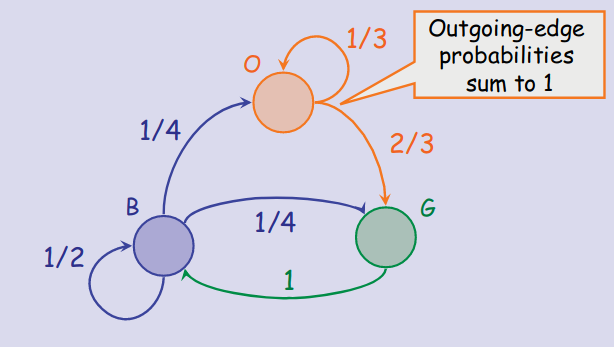
\includegraphics[width=0.8\textwidth]{../img/probgraph_example}
  \end{center}
\end{frame}

\begin{frame}
  \frametitle{Example: Gambler's Ruin}

  Imagine a game:
  \begin{itemize}
  \item With probability $p$ you win 1\$.
  \item With probability $q = 1-p$ you lose 1\$.
  \item You begin with $n$\$.
  \item What is the probability that you reach \structure{T\$}
      before you \alert{lose all?}.
  \end{itemize}
  
  \begin{center}
    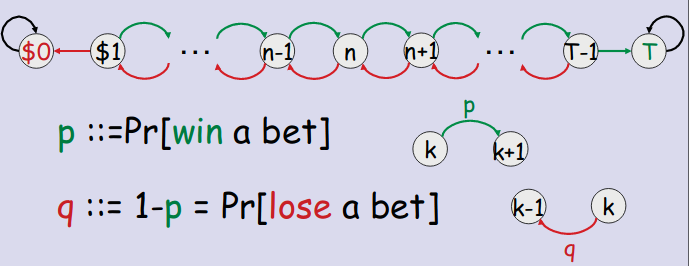
\includegraphics[width=0.9\textwidth]{../img/probgraph_gambler}
  \end{center}
\end{frame}

\begin{frame}
  \frametitle{Applications of Random Walk}

  {\larger
    \begin{itemize}
    \item {\bf Physics:} Brownian Motion
      \bigskip
      
    \item {\bf Finance:} Stock prediction/simulation, options
      \bigskip

    \item {\bf Computer Science:} Web Search, Clustering
    \end{itemize}
  }
\end{frame}

\begin{frame}
  \frametitle{Example: Coin Game -- HTH before TTH}


  {\larger
    
    {\bf Experiment:} You throw a coin many times, and keep track of
    \structure{the last three results}:

    \vfill

    \begin{itemize}
    \item If the sequence \structure{HTH} happens before the sequence
      \alert{TTH}, \structure{you win!}
      \bigskip

    \item If the sequence \alert{TTH} happens before the sequence
      \structure{HTH}, \structure{you lose!}
    \end{itemize}
    

    \bigskip

    What is the probability that you win this game?

  }
\end{frame}

\begin{frame}
  \frametitle{Example: Coin Game -- HTH before TTH}
  \begin{center}
    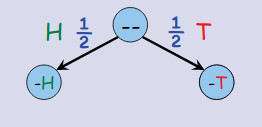
\includegraphics[width=0.8\textwidth]{../img/hth_1}
  \end{center}

  {\larger
    \begin{itemize}
    \item Pr[Win] = Pr[Win|--] = 1/2 Pr[Win|-H] + 1/2 Pr[Win|-T]
    \end{itemize}
  }
\end{frame}

\begin{frame}
  \frametitle{Example: Coin Game -- HTH before TTH}
  \begin{center}
    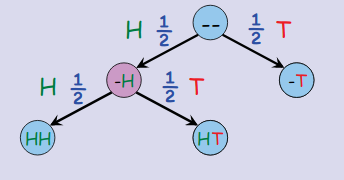
\includegraphics[width=0.8\textwidth]{../img/hth_2}
  \end{center}

  {\larger
    \begin{itemize}
    \item Pr[Win|-H] = 1/2 Pr[Win|HH] + 1/2 Pr[Win|HT]
    \end{itemize}
  }
\end{frame}

\begin{frame}
  \frametitle{Example: Coin Game -- HTH before TTH}
  \begin{center}
    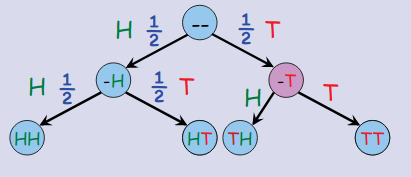
\includegraphics[width=0.8\textwidth]{../img/hth_3}
  \end{center}

  {\larger
    \begin{itemize}
    \item Pr[Win|-T] = 1/2 Pr[Win|TH] + 1/2 Pr[Win|TT]
    \end{itemize}
  }
\end{frame}

\begin{frame}
  \frametitle{Example: Coin Game -- HTH before TTH}
  \begin{center}
    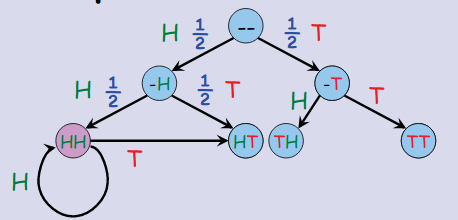
\includegraphics[width=0.8\textwidth]{../img/hth_4}
  \end{center}

  {\larger
    \begin{itemize}
    \item Pr[Win|HH] = 1/2 Pr[Win|HH] + 1/2 Pr[Win|HT]
    \end{itemize}
  }
\end{frame}

\begin{frame}
  \frametitle{Example: Coin Game -- HTH before TTH}
  \begin{center}
    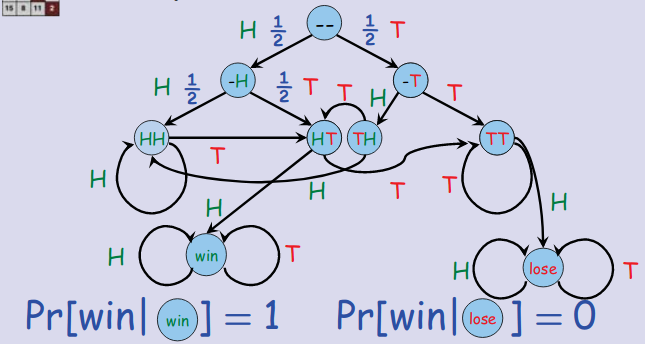
\includegraphics[width=0.8\textwidth]{../img/hth_5}
  \end{center}

  {\larger

    \bigskip

    And you can solve the system of linear equations for \structure{Pr[Win]}.
  }
\end{frame}

\subsection{Stationary Distributions}

\begin{frame}
  \frametitle{Stationary Distributions}

  \begin{center}
    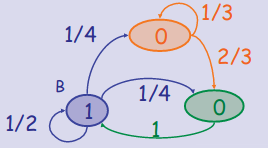
\includegraphics[width=0.4\textwidth]{../img/probgraph_walk}
  \end{center}

  \bigskip

  {\larger
  Suppose you start at {\bf B}: $(p_b = 1, p_o = 0, p_g = 0)$
  \bigskip

  What are the probabilities of each state: $(p_b', p_o', p_g')$ at
  the next step?
  }
\end{frame}

\begin{frame}
  \frametitle{Stationary Distributions}

  \begin{center}
    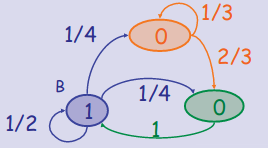
\includegraphics[width=0.4\textwidth]{../img/probgraph_walk}
  \end{center}

  \bigskip
  
  {\larger
    After 1 step, you follow the out-edges from B:
    \begin{itemize}
    \item $p_b' = p_b\cdot 1/2 = 1/2$
    \item $p_o' = p_b\cdot 1/4 = 1/4$
    \item $p_g' = p_g\cdot 1/4 = 1/4$
    \end{itemize}
    \structure{$(p_b', p_o', p_g') = (1/2, 1/4, 1/4)$}
  }
\end{frame}


\begin{frame}
  \frametitle{Stationary Distributions}

  \begin{center}
    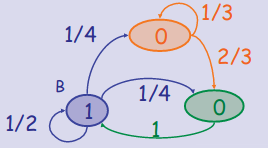
\includegraphics[width=0.4\textwidth]{../img/probgraph_walk}
  \end{center}

  \bigskip
  
  {\larger After 2 steps: \alert{$(p_b'', p_o'', p_g'')$} from $(p_b' = 1/2,
    p_o' = 1/4, p_g' = 1/4)$
    \begin{itemize}
    \item $p_b'' = p_b'\cdot 1/2 + p_g'\cdot 1 = 1/2$
    \item $p_o'' = p_b'\cdot 1/4 + p_o'\cdot 1/3 = 5/24$
    \item $p_g'' = p_b'\cdot 1/4 + p_o'\cdot 2/3 = 7/24$
    \end{itemize}
    \structure{$(p_b'', p_o'', p_g'') = (1/2, 5/24, 7/24)$}
  }
\end{frame}

\begin{frame}
  \frametitle{Edge Probability Matrix}

  {\larger
  The \structure{edge probability matrix} is the same as the adjacency
  matrix, \alert{using edge probabilities instead of zeroes and ones}.
  
  \bigskip
  
  \begin{equation*}
    M = \left(\begin{matrix}
    1/2 & 1/4 & 1/4 \\
    0 & 1/3 & 2/3 \\
    1 & 0 & 0 \\
    \end{matrix}\right)
  \end{equation*}

  \bigskip
  
  We can use the \structure{edge probability matrix} to calculate the
  walk state after $i$ steps.
  }
\end{frame}

\begin{frame}
  \frametitle{Edge Probability Matrix: Usage}

  {\larger

    You can use the \structure{edge probability matrix} to calculate the
    state on the next step:

    \bigskip

    \begin{equation*}
      (p_b,p_o,p_g)\cdot M = (p_b',p_o',p_g')
    \end{equation*}
  }
\end{frame}

\begin{frame}
  \frametitle{Stable Distribution}

  {\larger

    What is the graph state at \structure{step t}?
    
    \begin{equation*}
      (p_b,p_o,p_g)\cdot M^t = (p_b^t,p_o^t,p_g^t)
    \end{equation*}
    
    \vfill
    
    What is the graph state at \structure{step $t\to\infty$}?
    
    \medskip

    \begin{itemize}
      \item Solve the system of equations:
    \end{itemize}
    \begin{equation*}
      \overrightarrow{s}\cdot M = \overrightarrow{s} \text{ and } \sum{s_i} = 1
    \end{equation*}
  }
\end{frame}

\begin{frame}
  \frametitle{Stable Distribution: Limitations}

  {\larger

    For some graphs, and some starting states, it may not be
    possible to find the stable distribution:

    \bigskip
    
    \begin{itemize}
    \item Graph may not converge to a stable distribution
      \bigskip

    \item Graph may have uncountable many stable distributions
      \bigskip

    \item Graph may have multiple stable distributions
    \end{itemize}

  }
\end{frame}


%% TODO: Add more information from the book
\subsection{Pagerank}

\begin{frame}
  \frametitle{Google Webpage Ranking}

  {\larger

    \begin{itemize}
    \item Which webpages are more important?
      \bigskip

    \item \structure{Model of the Internet:}\\
      Users \structure{click randomly} on links in a webpage.\\
      Item sometimes the user \structure{starts over} from a new page
      \bigskip

    \item A page is ``more important'' if it is viewed more time.\\
      \hfill (probability in a ``random walk'')
    \end{itemize}    
  }
\end{frame}

\begin{frame}
  \frametitle{A random walk for the internet}

  {\larger
    \begin{itemize}
    \item Represent the internet as a \structure{Directed Graph} (DiGraph)
      \bigskip
      
    \item Each \structure{webpage is a vertice, $V_i$}
    \item A link from page $V_i$ to page $V_j$ is \structure{an Edge $E_{ij}$}
      \bigskip

    \item Identical probability for each edge out of $V_i$:
      \structure{Pr$[E_{ij}] = 1/\text{deg}(V)$}
    \end{itemize}
  }
\end{frame}

\begin{frame}
  \frametitle{A random walk for the internet}

  {\larger
    To model \structure{starting over}:
    \vfill
    
    \begin{itemize}
    \item Add a \structure{``super node''} to the graph;
      \bigskip
      
    \item The \structure{super node} has an edge from it to
      \structure{every other node};
      \bigskip
      
    \item Every other node has \structure{an edge back to the
      supernode};\\
      \bigskip
      
      \hfill (maybe with customized probabilities)
    \end{itemize}
  }
\end{frame}

\begin{frame}
  \frametitle{A random walk model of the internet}
  \begin{center}
    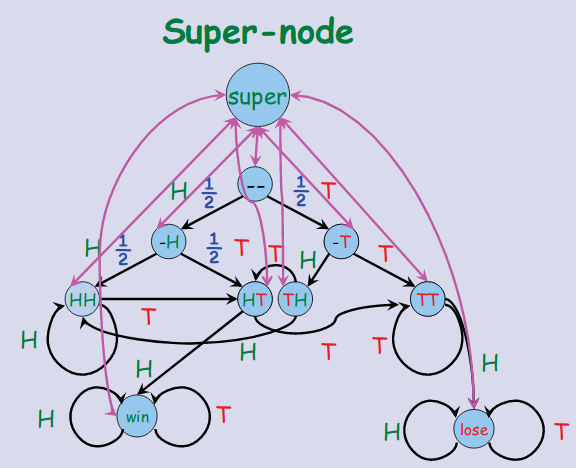
\includegraphics[width=0.7\textwidth]{../img/pagerank_supernode}
  \end{center}
\end{frame}

\begin{frame}
  \frametitle{Pagerank}

  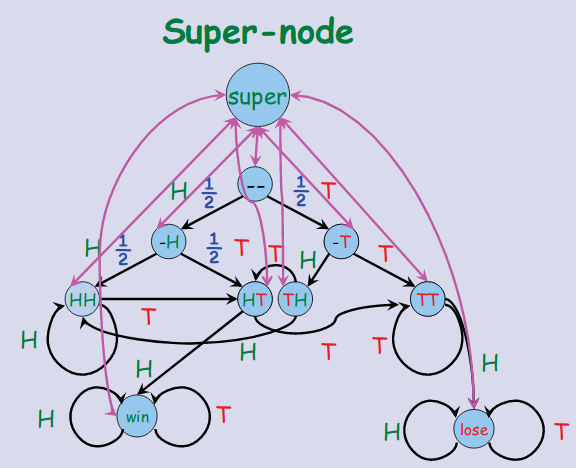
\includegraphics[width=0.3\textwidth]{../img/pagerank_supernode}

  \bigskip

  {\larger
  \begin{itemize}
  \item Compute the \structure{stationary distribution} $\overrightarrow{s}$
    \begin{equation*}
      \text{Pagerank}(V) ::= s_V
    \end{equation*}
    \bigskip

  \item Rank page $V_i$ above page $V_j$ when:
    \begin{equation*}
      s_v > s_w
    \end{equation*}
  \end{itemize}
  }
\end{frame}

\begin{frame}
  \frametitle{Pagerank}

  Resistant to \alert{scamming}:
  \begin{itemize}
  \item Creating \alert{fake nodes pointing to self} does not help.
  \item Adding links to other nodes has \alert{Diminishing Returns}
  \end{itemize}
  \vfill

  Importance of \structure{supernode}:
  \begin{itemize}
  \item Ensures \structure{unique stable distribution} $\overrightarrow{s}$
  \item Ensures that \structure{every initial condition $\overrightarrow{p}$} converges to $\overrightarrow{s}$ 
  \end{itemize}

  \vfill
  \hfill (Of course, Google's algorithm today has more tricks)
  
\end{frame}

\section{Sample Exam}

\begin{frame}
  \frametitle{Exam Information}

  \begin{itemize}
  \item Sample Exam
  \item Class Evaluation
  \item Final Exam
  \item Grades    
  \end{itemize}
\end{frame}

\begin{frame}
  \frametitle{Sample Exam \& Class Evaluation}

  \begin{itemize}
  \item The sample exam is an idea of what kind of questions are asked in the final exam.
    \bigskip
    
  \item The sample exam {\bf will not} be graded.
    \bigskip
    
  \item Please feel free to ask for help in the sample exam.
    \bigskip

  \item Please complete the Class Evaluation too.    
  \end{itemize}
\end{frame}

\begin{frame}
  \frametitle{Final Exam}

  \begin{itemize}
  \item {\bf You can bring:} 1 note page\\
    \hfill(A4, front and back, with name and student number)
    \bigskip
    
  \item {\bf You can bring:} Dictionary, Electronic Dictionary,
    \structure{calculator}
    \bigskip
    
  \item \alert{{\bf You can NOT use:}} Textbook, class slides,
    computer.
  \end{itemize}
\end{frame}

\begin{frame}
  \frametitle{Grades}
  \begin{itemize}
  \item \structure{Assignment Grade:} Before the Final Exam
    \bigskip
    
  \item \structure{Final Exam Grade:} Before 1/4
    \bigskip
    
  \item \structure{Grade Questions:} Until 1/11
  \end{itemize}
\end{frame}

\end{document}
